%!TEX root = ./main.tex
\chapter{LANDASAN TEORI}

\section{Tinjauan Pustaka}
\subsection{Lorem}
\lipsum
\begin{tabel}[h]
	\caption{Apakah ini}
	\begin{tabular}{ccc}
		No & What & Ouh \\ \hline
		1 & ? & as
	\end{tabular}
\end{tabel}


%
\subsection{Mel Frequencies Cepstral Coefficients}
Salah satu teknik yang digunakan pada proses ektraksi fitur adalah Mel Factor Cepstral Coefficients (MFCC). \cite{Setiawan2011} menjelaskan, MFCC adalah proses pengubahan sinyal suara yang didasarkan pada variasi bandwidth kritis terhadap frekuensi yang dapat diterima telinga manusia yang berupa filter yang bekerja secara logaritmik pada frekuensi tinggi dan bekerja secara linear pada frekuensi tingkat rendah. Filter ini berguna untuk menangkap karakteristik fonetis yang penting dari sinyal gelombang suara. Untuk beradaptasi dengan kondisi telinga manusia, karakteristik ini digambarkan dalam skala mel-frekuensi yang berupa frekuensi linear di bawah 1000Hz dan frekuensi logaritmik di atas 1000Hz. Proses pengubahan data sinyal gelombang menjadi mffc dapat dilihat pada gambar di bawah ini:
\begin{figure}[H]
	\centering
	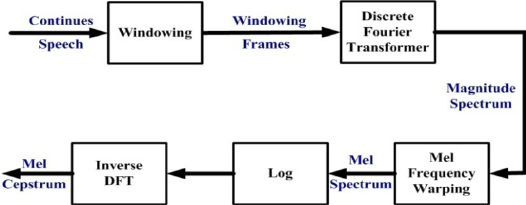
\includegraphics[width=0.7\linewidth]{Gambar/skema-mfcc}
	\caption{Alur kerja MFCC}
	\label{fig:skema-mfcc}
\end{figure}

\subsubsection{Frame Blocking}
Frame blocking adalah proses membagi sinyal gelombang suara yang panjang menjadi bagian-bagian kecil. Ucapan yang terdiri atas S sample $ X(S) $ dibagi menjadi beberapa frame yang berisi \textit{N} sample, masing-masing frame dipisahkan oleh M sample dengan $ M < N $. Frame pertama terdapat sampel \textit{N} pertama. Frame kedua dimulai \textit{M} sampel setelah permulaan frame pertama, sehingga frame pertama tumpang tindih (\textit{overlap}) dengan frame kedua sebanyak $ M-N $ sampel. Proses ini terus berlanjut hingga seluruh sampel berada dalam frame.
\subsubsection{Windowing}
Setelah proses frame blocking selesai dilakukan, proses windowing dilakukan agar meminimalkan diskontinuitas sinyal pada permulaan dan akhir setiap frame. Konsep windowing adalah meruncingkan sniyal mendekati angka nol pada permulaan dan akhir setiap frame. Jika window didefinisikan sebagai $ w(n), 0 \leq n \leq N-1s$ dengan N adalah jumlah sampel dalam tiap frame, maka hasil dari proses ini adalah gelombang:
\begin{equation}
y(n) = x(n) \cdot w(n), 0 \leq n \leq N -1
\end{equation}
dengan $y(n)$ = sinyal hasil \textit{windowing} ke-\textit{n}
$x(n)$ = nilai sampel ke-\textit{n}
$w(n)$ = nilai window ke-\textit{n}
\textit{N} = jumlah sampel dalam frame
Secara empirik penggunaan jenis window dalam mfcc adalah menggunakan hamming window dengan persamaan,
\begin{equation}
w(n) = 0.54 + 0.46 \cos \left( \frac{2\pi n}{N - 1} \right), 0 \leq n \leq N -1
\end{equation}

\subsubsection{Fast Fourier Transform}
Setelah dilakukan windowing dengan hamming window, langkah selanjutnya adalah mengubah sampel dari domain waktu ke domain frekuensi. Untuk melakukan ini kita akan mengimplementasi persamaan \textit{Discrete Fourier Transform} (DFT) ke dalam Fast Fourier Transform. Sampel yang sudah didapat kemudian dimasukkan ke dalam persamaan
\begin{equation}
f(n) =\sum_{k=0}^{N-1} y_{k} e^{-2\pi jkn / N}, n = 0,1,2, \ldots ,N-1
\end{equation}
\subsubsection{Mel-Frequency Wrapping}
Persepsi telinga manusia dalam freskuensi suara dalam sinyal ucapan tidak mengikuti skala linear. Maka, untuk setiap nada dengan frekuensi sesungguhnya \textit{f} dalam Hz, sebuah pola diukur dalam sebuah skala yang disebut 'mel'. Skala 'mel frekuensi' adalah skalan frekuensi linear di bawah 1000 Hz dan skala logaritmik di atas 1000 Hz.
Skala ini didefinisikan oleh %% cari paper tentang stanley smith 
sebagai :
\begin{equation}
mel(f) = 2595 \cdot \log_{10} \left(1 + \frac{f}{700}\right)
\end{equation}
Pendekatan yang mudah dipahami untuk simulasi spektrum dalam skala mel adalah dengan menggunakan \textit{filter bank}\label{idx:filbank} yang diletakan secara seragam dalam skala mel yang ditunjukkkan pada gambar di bawah ini:
\begin{figure}[H]
	\centering
	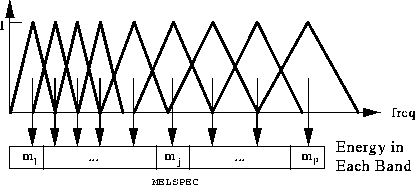
\includegraphics[width=0.7\linewidth]{Gambar/skala-mel}
	\caption{Skala Mel pada Filterbank}
	\figsource{Sumbernya dimana}
	\label{fig:skala-mel}
\end{figure}


Jika spektrum F[N] adalah masukan dalam proses ini, maka hasil proses ini adalah spektrum M[N] yang merupakan spektrum F[N] yang telah diubah dengan nilai berupa \textit{power output} dari filter-filter ini. Koefisien spektrum mel dinyatakan dalam K dan secara khusus ditentukan dengan nilai 20.
Dalam \textit{mel-frequency wrapping}, sinyal yang dihasilkan dalam proses sebelumnya dikelompokkan ke dalam berkas filter segitiga tersebut. Maksud dari pengelompokkan dalam hal ini adalah penjumlahan dari setiap nilai dari FFT dikalikan dengan\textit{gain filter} yang bersesuaian. Maka setiap kelompok memiliki sejumlah bobot energi sinyal yang ditampilkan sebagai $ m_1 \ldots m_p $ seperti dalam gambar.
\subsubsection{Cepstrum}
Ceptrum adalah istilah yang digunakan untuk kebalikan dari \textit{spectrum}. Untuk mendapatkan informasi dari sebuah suara yang diucapkan oleh manusia biasa menggunakan Ceptrum. Hasil dari proses \textit{mel-frequency wrapping} yang telah dilakukan, akan dikonvesi menggunakan \textit{Discrete Cosine Transform} (DCT) untuk mendapatkan nilai dari Mel-Frequency Ceptrum Coefficients (MFCC).
Secara formal MFCC didefinisikan sebagai alihragam kosinus dari logaritma \textit{short-term power spectrum} yang dinyatakan dalam skala mel-frekuensi. Jika $S_k, k = 1,2, \ldots, K$ dinyatakan sebagai \textit{mel power spectrum coefficients}, Minh N.Do mendefinikan koefisien dari MFCC sebagai:
\begin{equation}
c_n = \sum_{k=1}^{K} (log S_k) \cos\left[ n(k- \frac{1}{2}) \frac{\pi}{K} \right] , n = 1,2, \ldots ,K
\end{equation}


\subsection{i-Vector}
i-Vector Extraction atau ekstraksi i-vector adalah sistem yang memproyeksikan sekuens dari vektor (biasanya cepstral coeffiecients) yang diperoleh dari ucapan, $ O = \lbrace o_t\rbrace_{t=1}^{N} $ dengan $ o_t \in \mathbf{R}^F $, ke dalam vektor dengan panjang tertentu $ \eta \in \mathbf{R}^D $. Untuk melakukan itu, sebuah Gaussian Mixture Model dengan K komponen , $ \lambda = ( \lbrace w_k \rbrace, \lbrace m_k \rbrace,\lbrace \Sigma_k \rbrace) $ yang didenotasikan sebagai Universal Background Model (UBM) digunakan untuk mengambil Baum-Welch statistik dari setiap ucapan. Selanjutnya, sebuah supervector $ \theta = [ \theta_1^T, \ldots,  \theta_K^T]^T \in \mathbf{R}^{FK}$ dibangun dengan cara menyatukan statistik tingkat pertama dari masing-masing komponen \textit{mixture} dengan asumsi mengikuti persamaan model linear standard dalam bentuk:
\begin{equation}
\theta = m+\mathtt{T}x 
\end{equation}
dimana, supervector $ m \in \mathbf{R}^{FK} $ diperoleh dari UBM, $ T \in \mathbf{R}^{FK \times D}$ berupa matriks dari kolom-kolom rank rendah yang diperluas dalam subruang dimana kebanyakan informasi khas dari masing-masing pembicara, dan  sebagai variabel laten dari distribusi normal. Untuk setiap ucapan, i-vector $\eta$ diperoleh sebagai peta dari  perkiraan posisi dari. Subruang yang diperluas oleh  diperoleh dari himpunan data representatif yang besar  dari proses estimasi yang dilakukan oleh Machine Learning.
\subsection{One Time Password}


\newpage
\section{Penelitian Sebelumnya}
\begin{enumerate}
	
	\item Penulis: Jos\`{e} Port\^{e}lo, Bhiksha Raj, Alberto Abad dan Isabel Trancoso\\ 
	Tahun: 2014\\
	Judul: \textit{Privacy-Preserving Speaker Verification using Secure Binary Embedding}  \\
	\lipsum[1]
	
	\item Penulis: Lee Mun Kyu, Nam Hyeongjin dan Kim Dong Kyu\\
	Tahun: 2017\\
	Judul: \textit{Secure Biomodal PIN-Entry Method using audio signals}  \\
	\lipsum[2]
	
	\item Penulis : Reshma Begum, Basavaraj Gadgay, Veeresh Pujari, Pallvi B. V. \\
	Tahun : 2017 \\
	Judul : \textit{Security of ATM System Using Biometric and OTP}
	\lipsum[3]
	
	\item Penulis : Aleluya dan Vicente\\
	Tahun : 2018 \\
	Judul : \textit{FacetureID: face and hand gesture multi-factor authentication using deep learning.}\\
	\lipsum[4]
	
	\item Penulis : Junaedi Fahmi\\
	Tahun: 2018\\
	Judul : Pengunaan \LaTeX untuk mengurangi kegalauan skripsi\\
	\lipsum[5]
\end{enumerate}

\begin{penelitianterkait}
	\captionof{table}{Perbedaan Penelitian }
	\begin{longtable}{|p{0.5cm} | p{3.2cm} | p{3.2cm} | p{7cm} | p{7cm} | }
		\hline
		\thead{No} & \thead{Penulis (Tahun)} & \thead{Judul} & \thead{Hasil} & \thead{Keterangan} \\ \hline
		1          &                         &               &               &                    \\ \hline
		2          &                         &               &               &                    \\ \hline
		3          &                         &               &               &                    \\ \hline
		4          &                         &               &               &                    \\ \hline
		5          &                         &               &               &                    \\ \hline
	\end{longtable}
\end{penelitianterkait}

\subsection{Penelitian Sekarang}

Penelitian sekarang adalah menguji skema otentikasi menggunakan dua faktor. Faktor pertama dengan menggunakan OTP dan faktor kedua dengan biometrik. Biometrik yang digunakan berupa suara. Proses verifikasi menggunakan suara menggunakan teknologi Jaringan Saraf Tiruan dengan topologi yang disesuaikan.

\begin{comment}
\bibliography{daftarpustaka}
\end{comment}